\documentclass[twoside,11pt]{article}
\usepackage{jair, theapa, rawfonts, amsmath}
\usepackage[utf8]{inputenc}
\usepackage{graphicx}
\usepackage{subfig}
\usepackage{bigstrut}
\DeclareMathOperator{\sign}{sign}
\DeclareMathOperator{\subjectto}{subject to}

%\jairheading{1}{1993}{1-15}{6/91}{9/91}
\ShortHeadings{Predicting High School Dropouts}
{Weiss}
\firstpageno{1}

\begin{document}

\title{Predicting High School Dropouts}

\author{\name Adam Weiss \email aweiss17@jhu.edu \\
       \addr Johns Hopkins University,
       Baltimore, MD}

% For research notes, remove the comment character in the line below.
% \researchnote
\maketitle

\begin{abstract}
This paper describes an approach to creating a predictive model for detecting
high school dropouts before they actually drop out.  This model is developed
using machine learning on the National Center for Education Statistics 2009
Educational Longitudinal Survey.  Because the high dimensionality of the
dataset, principal component analysis is performed on the dataset to reduce its
dimensionality.  A multi-layer artificial neural network, $k$-nearest
neighbors, a support vector machine with a radial basis function kernel and a
support vector machine with a polynomial kernel are compared to determine which
has the best classification accuracy.  The results show that the neural network
has the highest accuracy, however it is only significantly higher than
$k$-nearest neighbors.
\end{abstract}

\section{Introduction}
\label{Introduction}
Dropping out of school can have dire consequences for the remainder of a
student's life.  Compared to students who graduate high school, dropouts are
much more likely to be living in poverty, unhealthy, unemployed, in prison,
divorced, and have children who will also drop out from high school
\cite{Bridgeland:2006}.  On average, these students end up making \$1 million
less over their lifetimes than those who graduate
\cite{Education-Statistics:1992}.  Although high school graduation rates have
been improving nationally, 10 states have shown lower graduation rates over the
past decade \cite{Balfanz:2012}.  If students who are at risk of dropping out
could be flagged before they drop out, and some kind of intervention could be
performed to prevent those students from dropping out, much of these hardships
could possibly be avoided.  

This paper will use the 2009 dataset from the Education Longitudinal Study
(ELS) by the National Center for Education Statistics (NCES), which contains
almost 7000 variables for over 23,000 students \cite{Ingels:2013}. ELS is one
of many large longitudinal surveys by NCES. These surveys track students
starting from either ninth or tenth grade, depending on the survey, and follows
them through their adult life.  The 2009 survey analyzed in this paper includes
a survey of ninth graders in the 2009-2010 school year, and one follow-up in
the spring of 2012.  The sampling is representative of students in the United
States.  It includes students randomly selected from more than 900 schools from
all 50 states and the District of Columbia.  The data in the survey includes
information about the student, the student's parents, socioeconomic background,
the student's teachers, and more.  In this study, 8.43 percent of the students
dropped out of school.

This paper aims through the use of machine learning to form an accurate
predictive model of students who are at risk of dropping out.  The data will be
classified using multi-layer artificial neural networks, k-nearest neighbors
($k$-NN), and with support vector machines using either radial basis function
kernels and polynomial kernels.  The classification accuracy of the various
models will be compared against one another.  Principal component analysis
(PCA) will be performed on the dataset to reduce its dimensionality while still
being representative of the distribution.  This newly transformed dataset will
be used to build the various models and ultimately determine their
classification accuracy.

The hypothesis that will be tested in this paper is a SVM using a radial basis
function kernel will have better classification accuracy than a neural network,
$k$-NN, or a SVM with a polynomial kernel.  One argument for this hypothesis is
the convexity of the SVM hinge loss function will result in optimization that
will not become stuck in local minima and will result in the SVM having the
highest classification accuracy.  Conversely, neural networks do not have
guaranteed convexity and can therefore can have issues with becoming stuck in
local minima.  In addition, the soft-margin of the SVM class hyperplane can
control the sensitivity to outliers.  $k$-NN, which has a similar Euclidean
distance calculation to the radial basis function kernel of the SVM, does not
have an equivalent `slackness' parameter.  Also, it is generally accepted that
RBF kernels typically outperform polynomial kernels \cite{Chang:2010}.   

\section{Literature Review}

There have been several studies of student performance using a variety of
methods.  Below is a sampling of some recent research which includes
statistical analysis of dropout data along with applying machine learning to
student performance and student attrition.

Suhyun et al. (2011) \nocite{Suhyun:2011} investigated the change in high
school dropouts between the 1980s and 2000s.  In their paper, they used
statistical analysis on two NCES National Longitudinal Survey of Youth (NLSY)
surveys in the 1980s and the 2000s.  In their analysis, they discovered the
eight strongest factors contributing to student dropouts are: students with a
minority race, student gender, whether students lived with a biological parent
in the first year of the survey, the mother's permissiveness, number of
household members, whether the student lived in a metropolitan area, whether
the student lived in the south or west of the United States, and students who
were suspended from school at least once.  They then went on to analyze how
these factors have changed between the 1980s and the 2000s.

Kotsiantes' (2011) \nocite{Kotsiantis:2011} study examined a number of
regression techniques to attempt to predict students' grades.  Their dataset
used information about a student's background and previous grades to form a
predictive model of future performance.  They compared the performance of a
number of different classifiers including model trees, neural networks, linear
regression, locally weighted regression, and support vector machines.  They
found model trees had the best performance of the tested regression models.

Yadav et al. (2011) \nocite{Yadav:2011} performed a similar study to Kotsiantes
with the goal of predicting students' grades.  They used decision trees to
build a model of future performance based on previous behavior such as grades
from the previous semester, attendance, test grades, and more.  They found that
Classification and Regression Trees (CART) provided the best classification
performance with an overall accuracy of 0.5625.

Chen et al. (2007) \nocite{Chen:2007} analyzed performance assessment in
Web-based learning environments.  The goal was to be able to provide immediate
useful feedback regarding learning performance to the student.  Their approach
used a combination of four techniques: gray relational analysis (GRA), K-means
clustering scheme, fuzzy association rule mining, and fuzzy inference.  Their
results showed moderate performance with a maximum average accuracy of 0.7675.

Delen (2010) \nocite{Delen:2010} compared the results of multiple classifiers
at predicting freshmen student attrition in Oklahoma State University.  Using a
total of 29 variables that included age, high school GPA, SAT score, and fall
student loan amount, they found that a SVM resulted in the best overall
prediction accuracy of 0.8645.  They compared decision trees, artificial neural
networks, and logistic regression and SVMs in their paper.

Lykourentzou et al. (2009) \nocite{Lykourentzou:2009} attempted to predict
dropouts in e-learning courses using feed-forward neural networks, support
vector machines, and probabilistic ensemble fuzzy ARTMAP.  In their paper, they
used time-invariant along with time-varying attributes to form their models.
These variables include student demographics, prior academic performance,
gender, and grades on assignments.  They found that by at the start of a
course, they could predict dropouts with 85 percent accuracy and by the middle
of the course they reached 97 percent accuracy.  No one classifier performed
the best at all stages of the course, and each performed the best in at least
one stage of the course.

Pal (2012) \nocite{Pal:2012} conducted a study of predicting higher education
student dropouts in India using naïve bayes classifiers.  They found with only
17 variables such as overall high school GPA, family income, and parents'
occupations, they were able to predict dropouts with an accuracy of 0.917. 


\section{Experiments}

The NCES longitudinal surveys have a great wealth of information spread over a
number of years.  Unfortunately, processing the more than 7000 variables and
more than 23000 samples in the 2009 ELS survey using machine learning is
computationally expensive.  To reduce the computational cost of training this
large dataset, steps will be taken to reduce its dimensionality.  First,
variables that are restricted will be removed as this data cannot be used
publically.  Next, any variable with a variance of zero is removed as these
will not contribute to the model.  Also, variables with a maximum value of less
than zero are also removed as these indicate that information is missing for
some reason.  These reasons include the student is incapable of answering a
question or the student is unresponsive to a given question.

PCA will then be performed on the resulting dataset.  PCA helps to avoid the
``curse of dimensionality'' by effectively compressing the dataset and keep
only the most important information.  It does this through calculating the
eigenvalues of the covariance matrix \cite{Pearson:1901}.  The transformation
results in the variables being sorted by variance.  Only the variables with the
most variance will be used, and the remaining variables whose variance differ
by less than ten percent will be discarded.  Because PCA transforms the dataset
into a representation of the original data, direct comparison between the
transformed and original variables is difficult.

\subsection{$k$-Nearest Neighbor}
The first classifier to be tested is the $k$-nearest neighbor ($k$-NN)
classifier.  $k$-NN is a lazy learning, non-parametric method that only
computes classes on demand based off the $k$-nearest classes to a given sample
vector \cite{Cover:1967}.  Given a point $x_0$, the $k$ points $x_{(r)},
r=1,...,k$ nearest to $x_0$ are found and $x_0$ is classified based off the
majority vote among the $k$-nearest neighbors.  The nearest neighbors can be
found by calculating the Euclidian distance between points:
\begin{equation}
  d_{(i)} = ||x_{(i)} - x_0||
\end{equation}
This results in zero computational cost for training, however the expense is
deferred until the classification step.  This simple method has good non-linear
classification accuracy, however high-dimensionality, noisy inputs and
irrelevant attributes are problematic for $k$-NN.  This makes PCA or other
forms of dimensionality reduction quite important when using $k$-NN classifiers
with high-dimensional datasets.  The $k$ parameter for the algorithm will be
tuned through 10-fold cross validation.

\subsection{Artificial Neural Network}
Next, an artifical neural network will be tested.  Neural networks attempt to
model the nervous system using representations of neurons.  A network with one
input and output layer of neurons can perform only linear separation.
Therefore, a multi-layered feed-forward neural network will be used due to its
ability to approximate non-linear functions \cite{Werbos:1974}.  The network
that will be tested will have one input layer, one hidden layer, and one output
layer.  Random weights will be assigned to all units and a gradient descent
method will be used to optimize the weights.  The perceptrons in the network
will use the activity function $A_{j} = \sum_i \omega_{ij} x_{i}$ along with
the sigmoidal activation function, $\frac{1}{1 + e^{-x}}$.  The neural network
is trained via gradient descent, the derivative of the loss function.  The
weights are updated with the function:
\begin{equation}
  \Delta \omega_{ij} = \eta \delta_j x_i
\end{equation} 
where $\eta$ is the learning rate and $\delta_j x_i$ is:
\begin{equation}
  [1-x_j]x_j(\sum_k \delta_k w_{jk} x_i)
\end{equation}
Gradient descent works well for training, however it can have trouble with
getting caught in local minima as well as overfitting \cite{Rojas:1996}.  To
avoid overfitting, a weight decay parameter $\lambda$ will be introduced to
penalize large weights and therefore regularize the weight update function.
The resulting weight update is the following: 
\begin{equation}
  \Delta \omega_{ij} = \eta \delta_j x_i - \eta \lambda x_i % only \lambda 
\end{equation} 
The parameters of the network will be chosen through cross-validation.  These
parameters are the number of hidden units in the network and the weight decay
parameter $\lambda$.  The best combination of these parameters will be used to
test the performance of the final model.

\subsection{Support Vector Machine}
The third and final classifier to be tested is the support vector machine
(SVM).  Linear SVMs create a model to find a hyperplane that separates two
classes of points.  The hyperplane, modeled by the simple equation $f(x) = x^T
\beta + \beta_0 = 0$, attempts to maximize the margin $M$ between the two
classes.  The margin $M = \frac{1}{||\beta||}$ is on each side of the
hyperplane where $\beta$ is a unit vector $||\beta|| = 1$.  Therefore,
classification is achieved by $G(x) = \sign[x^T\beta + \beta_0]$, leading to
the optimization problem 
\begin{equation*}
  \begin{aligned}
  &\min_{\beta, \beta_1} &&||\beta|| \\
  &\text{subject to } && y_i (x_i^T \beta + \beta_0) \geq 1, i = 1,...,N.
  \end{aligned}
\end{equation*}

To handle the case when the classes may overlap one another, slack variables
$\xi = (\xi_1, \xi_2,...,\xi_N)$ may be introduced to define the amount of
error allowed across the hyperplane, leading to the new optimization problem  
\begin{equation}
  \min ||\beta|| \text{ subject to } \begin{cases}
    \; y_i(x_i^T\beta + \beta_0) \geq 1 - \xi_i \forall i,\\
    \; \xi_i \geq 0,\: \sum \xi_i \leq \text{constant}
  \end{cases}
\end{equation}

This ``constant'' is the cost parameter $C$ of training the SVM.  All together,
this works well for linearly separable classes, however it will not work for
more complicated class boundaries that are non-linear.  To solve this issue, a
kernel function may be used.  A popular kernel to use is the Gaussian radial
basis function (RBF).  On two inputs, $x$ and $x'$, the RBF kernel is:
\begin{equation}
  K(x, x') = \exp(-\gamma||x - x'||^2)
\end{equation}                          % professor said polynomial kernels ar
% also popular and should maybe be evaluated as well
The solution to the hyperplane can be transformed to use a kernel function using the equation
\begin{equation}
  \hat{f}(x) = \sum_{i=1}^N\hat{\alpha_i} y_i K(x,x_i) + \hat{\beta}_0
\end{equation}
The result is a hyperplane that will curve with the class boundary.  Training
will be tuned using the cost parameter $C$ using 10-fold cross validation.

Another popular kernel is the polynomial kernel, represented by the following:

\begin{equation}
  K(x, x') = (1 + \lambda \langle x, x' \rangle)^d
\end{equation}
For the polynomial kernel, the degree parameter $d$, the cost parameter $C$, and
the scale parameter $\lambda$ will be tuned using 10-fold cross validation.

\subsection{Evaluation}

The four classifiers mentioned above, artificial neural network (denoted NN),
$k$-nearest neighbors (denoted KNN), and support vector machine with RBF
(denoted SVMR) and polynomial kernels (denoted SVMP), will be compared in terms
of overall classification accuracy and area under the receiver operator
characteristic (ROC) curve \cite{Zweig:1993}.  The tuning of the various
parameters will be presented to show how they affect overall classification
accuracy.  The parameters with the highest accuracy will be chosen, and this
configuration will be evaluated to determine the statistical significance of
the differences between classifiers.

\subsection{Results}
\begin{table}[htbp]
  \centering
  \caption{Accuracy, Area Under ROC, Sensitivity, and Specificity of the models}
    \begin{tabular}{rrrrr}
      \hline
    & Accuracy & ROC   & Sensitivity  & Specificity \\
\hline    
    NN    & 0.9396 & 0.8303 & 0.9957 & 0.3263 \\
    KNN   & 0.9340 & 0.7312 & 0.9988 & 0.2289 \\
    SVMR  & 0.9391 & 0.7937 & 0.9984 & 0.2954 \\
    SVMP  & 0.9394 & 0.793 & 0.9984 & 0.2963 \\
    \hline
    \end{tabular}%
  \label{tab:roc}%
\end{table}
Figure \ref{fig:bplot} and corresponding Table \ref{tab:roc} shows the
accuracy, the area under the ROC curve, the sensitivity, and the specificity of
the four classifiers.  NN had the highest accuracy, ROC value, and highest
specificity.  Table \ref{tab:Accuracypvalues} shows the differences in accuracy
between models above the diagonal along with the corresponding p-values with
Bonferroni correction (see \citeA{Bonferroni:1935}) below the diagonal.  This
table shows that while NN had the overall highest accuracy, the difference was
not significant over SVMR and SVMP, however NN did perform significantly better
than KNN.  SVMR was hypothesized to have the highest accuracy, however this was
not the case.  SVMP had slightly higher accuracy, however the difference is not
significant.  The accuracy between the classifiers was very close.

Table \ref{tab:ROCpvalues} shows the differences in area under the ROC curves
above the diagonal along with the corresponding p-values with Bonferroni
correction below the diagonal.  The difference between NN and the next highest
ROC value, SVMP, was significant with a p-value of 0.0046.  The differences
between ROC values was much greater than the differences in overall accuracy.
This corresponds with the greater variance in specificity.  All models had very
high sensitivity, however NN had the highest specificity.  Consequently, the
classifiers will most likely have very few false negatives, however there will
be many false positives identified.  That being said, it is better to falsely
identify a child as a potential drop out than to not identify chilren who are
likely to drop out.


\begin{figure}[htbp] 
  \centering
  \caption{Accuracy, ROC, Sensitivity, and Specificity Box Plots}
  \subfloat[]{\label{fig:bplotb}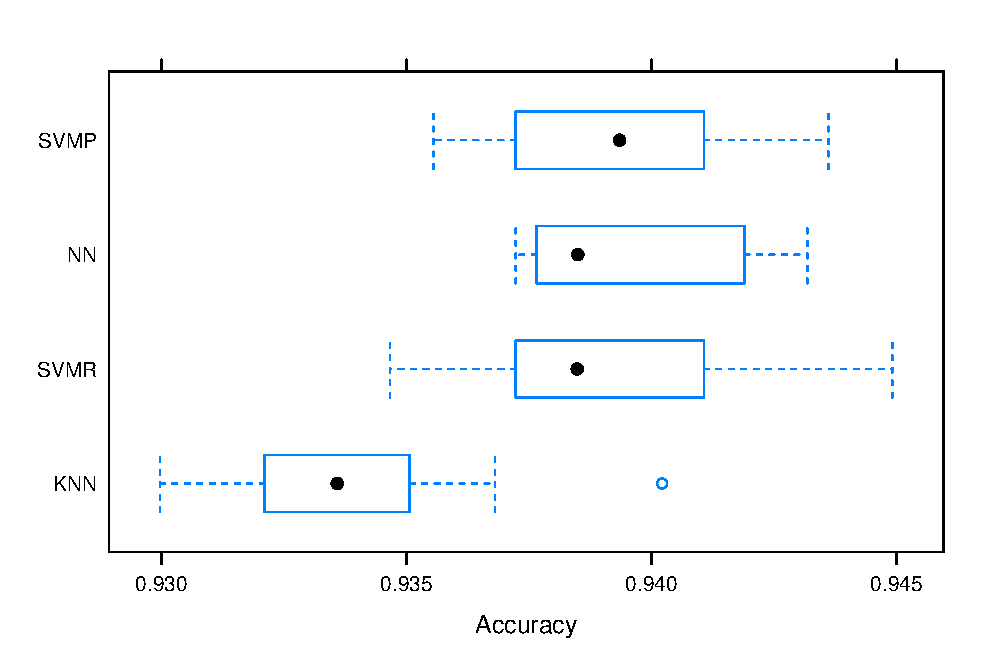
\includegraphics[scale=0.7]{accuracy.pdf}} \\
  \subfloat[]{\label{fig:bplota}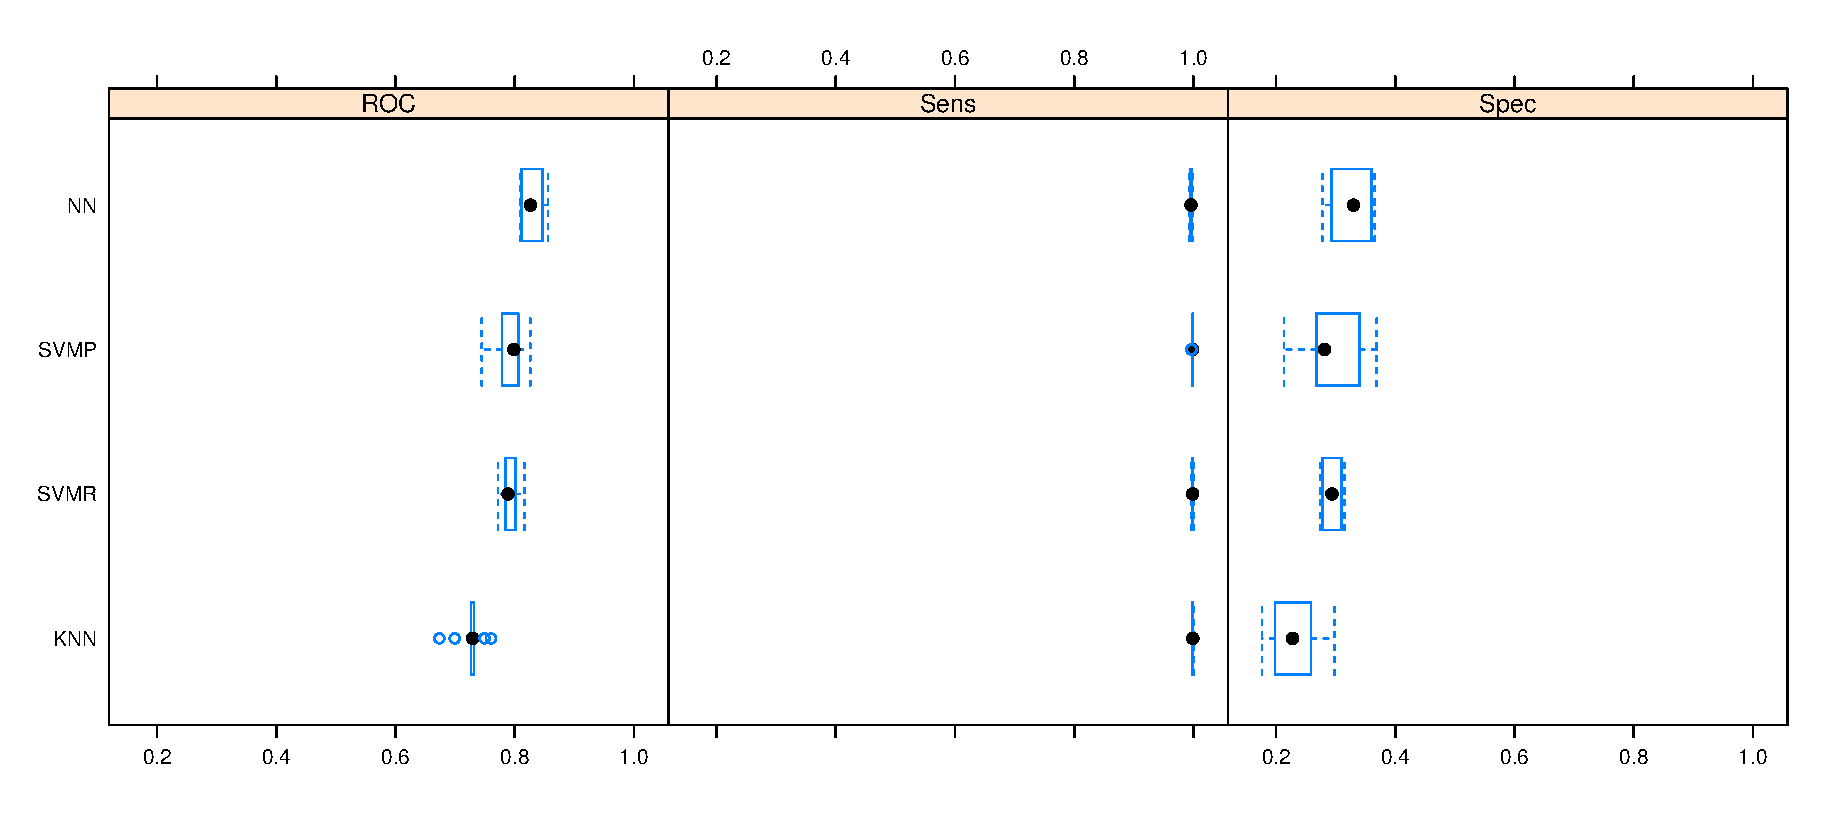
\includegraphics[scale=0.5]{bplot.pdf}} 
  \label{fig:bplot}
\end{figure}

Figure \ref{fig:tuning} shows the parameter selection for the four models.
Only one hidden unit was required for the NN model, along with a weight decay
$\lambda$ of 0.1.  Unfortunately, the NN model had issues with training more
than 7 hidden units, and it is possible that better performance could have been
obtained from more hidden units.  However, the overall trend was reduced
performance with additional hidden units.  KNN performed best with 10 nearest
neighbors with an accuracy of 0.9340.  More neighbors may have improved the
performance slightly, however it appears it is leveling off in Figure
\ref{fig:knn}.  SVMR performed best with a cost $C$ of 0.5 resulting in an
accuracy of 0.9391.  Finally, SVMP saw its best performance with a cost $C$ of
0.25, a scale of 0.01, and a degree 2 resulting in an accuracy of 0.9394.  

\begin{table}[ht]
\centering
\caption{Above the diagonal are the differences between model accuracy and
  below are the p-values with Bonferroni correction}
\begin{tabular}{rrrrr}
  \hline
 & NN & KNN & SVMR & SVMP \\ 
  \hline
NN &  &  0.0055522 &  0.0004271 &  0.0001278 \\ 
  KNN & 0.004984 &  & -0.0051251 & -0.0054243 \\ 
  SVMR & 1.000000 & 0.038251 &  & -0.0002993 \\ 
  SVMP & 1.000000 & 0.032182 & 1.000000 &  \\ 
   \hline
\end{tabular}
\label{tab:Accuracypvalues}
\end{table}

\begin{table}[htbp]
\centering
\caption{Above the diagonal are the differences between ROCs and below are the
  p-values with Bonferroni correction}
\begin{tabular}{rrrrr}
  \hline
 & NN & KNN & SVMR & SVMP \\ 
  \hline
NN &  &  0.1006253 &  0.0380372 &  0.0387978 \\ 
  KNN & 1.518e-07 &  & -0.0625881 & -0.0618274 \\ 
  SVMR & 7.805e-05 & 7.925e-06 &  &  0.0007607 \\ 
  SVMP & 0.0045639 & 0.0005211 & 1.0000000 &  \\ 
   \hline
\end{tabular}
  \label{tab:ROCpvalues}
\end{table}

\begin{figure}[htbp] 
  \centering
  \caption{Tuning Parameters for Classfication Models}
  \subfloat[NN]{\label{fig:nnet}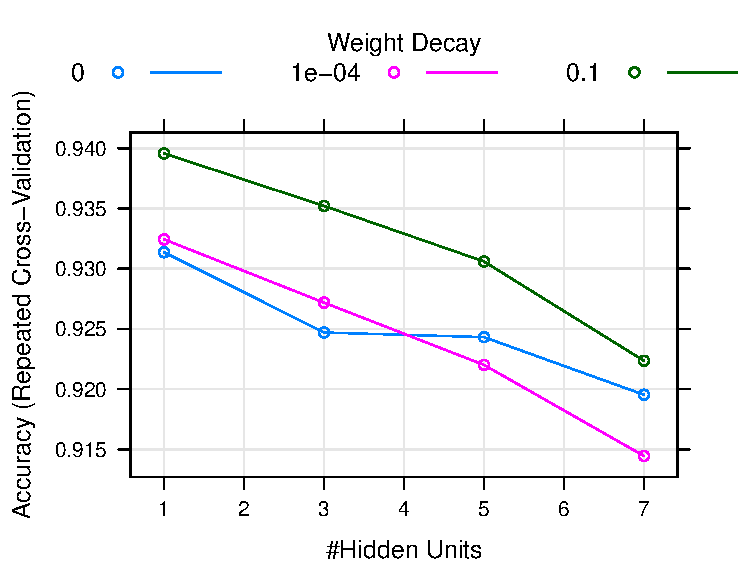
\includegraphics[scale=0.6]{nnplot2.pdf}}
  \subfloat[KNN]{\label{fig:knn}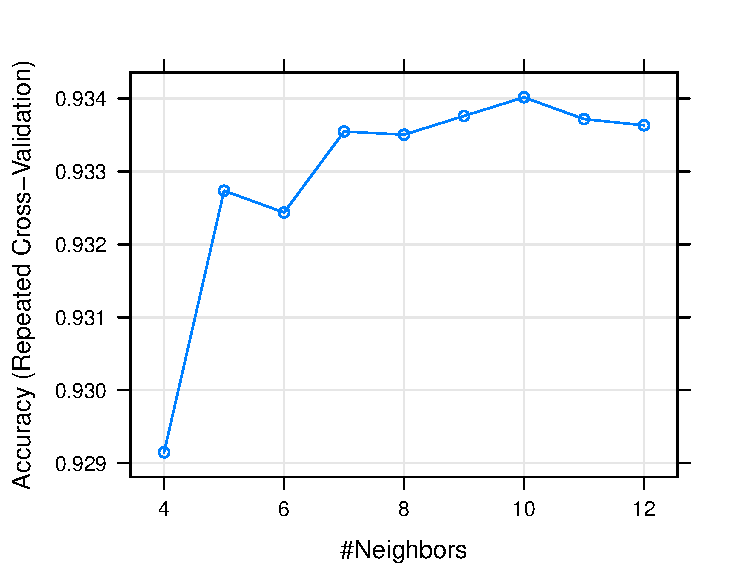
\includegraphics[scale=0.6]{knnplot2.pdf}} \\
  \subfloat[SVMR]{\label{fig:svmr}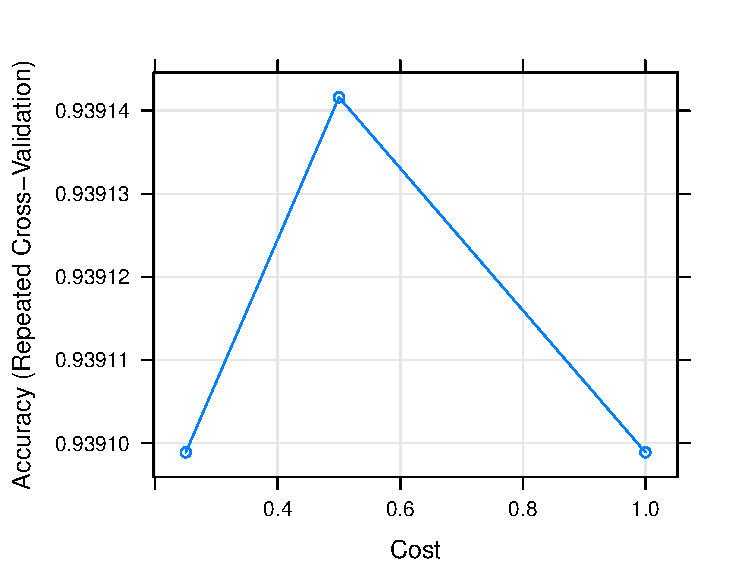
\includegraphics[scale=0.6]{svmrplot2.pdf}} 
  \subfloat[SVMP]{\label{fig:svmp}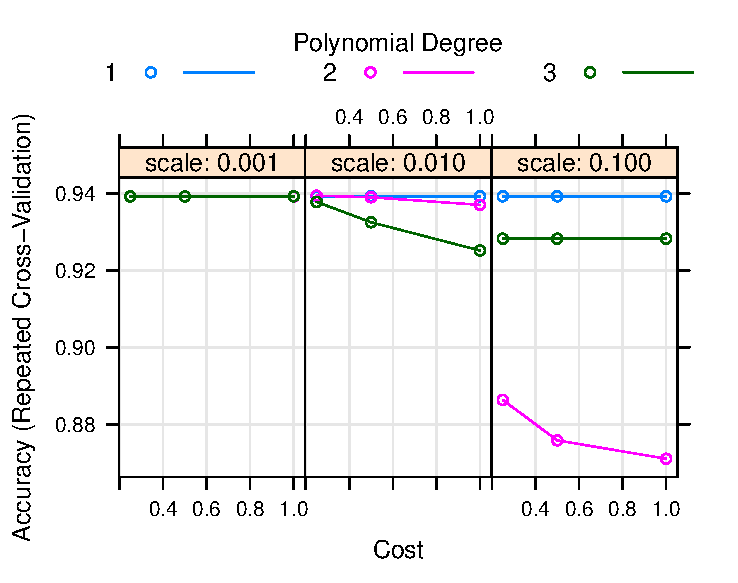
\includegraphics[scale=0.6]{svmpolyplot2.pdf}}
  \label{fig:tuning}
\end{figure}

\section{Conclusion}

This paper attempted to train four different models, NN, KNN, SVMR, and SVMP,
on the 2009 Educational Longitudinal Study with the goal of predicting if
students would drop out of high school.  PCA was applied to the dataset because
of its high dimensionality.  The classifier with the highest accuracy, NN, did
not perform significantly better than SVMR or SVMP.  However, NN did have a
significantly higher area under the ROC curve than all other classifiers.  The
main contribution of this paper shows that machine learning can be used to
detect high school drop outs before they occur with relatively high accuracy
and with few false negatives, however there will be some false positives.

This paper showed promising results, however there is much more work that can
be done.  More advanced classifiers can be used, such as state of the art
ensemble classifiers, to hopefully provide more accurate prediction of drop
outs.  Bayesian networks may be advantageous in identifying dependent
relationships between variables.  Another area of future work is to go one step
further and learn a Markov decision process to determine a policy of actions to
help prevent the student from dropping out.  Similar ideas could also be
applied to identify other potential risks in students, such as identifying
students who may not go on to college.  There are many more areas where machine
learning could be applied to education.  

%\vskip 0.2in
\bibliography{bibliography}
\bibliographystyle{theapa}

\end{document}
